%!TEX root = ../thesis.tex
%*******************************************************************************
%****************************** Third Chapter **********************************
%*******************************************************************************
\chapter{Main Methodologies}


\section[Experimentations]{Experimentations}

The devices investigated in this thesis were developed by the Electronic Materials and Devices group in the department. Despite the fact that the fabrication process was described in detail here for completeness, the tasks described here were not personally carried out, so all credit goes to the rest of the research group.


\subsection[Device Characteristics]{Device Characteristics}

\noindent The device investigated in this thesis has a metal-insulator-metal (MIM) structure and is manufactured on a silicon wafer. A thick silicon dioxide layer is thermally accumulated onto the wafer preparatory to the bottom electrode to prevent interactions between the bottom metal contact and the wafer. After that, the bottom electrode and thin film oxide are deposited unpatterned throughout the whole sample. Finally, during the deposition process, the top electrical contacts are patterned into squares with sides varying from $200\mu m$ to $800\mu m$ in Figure \ref{fig:3a}. Photolithography is not employed for patterning since a contact mask is used. \\

\begin{figure}[htbp!] 
    \centering    
    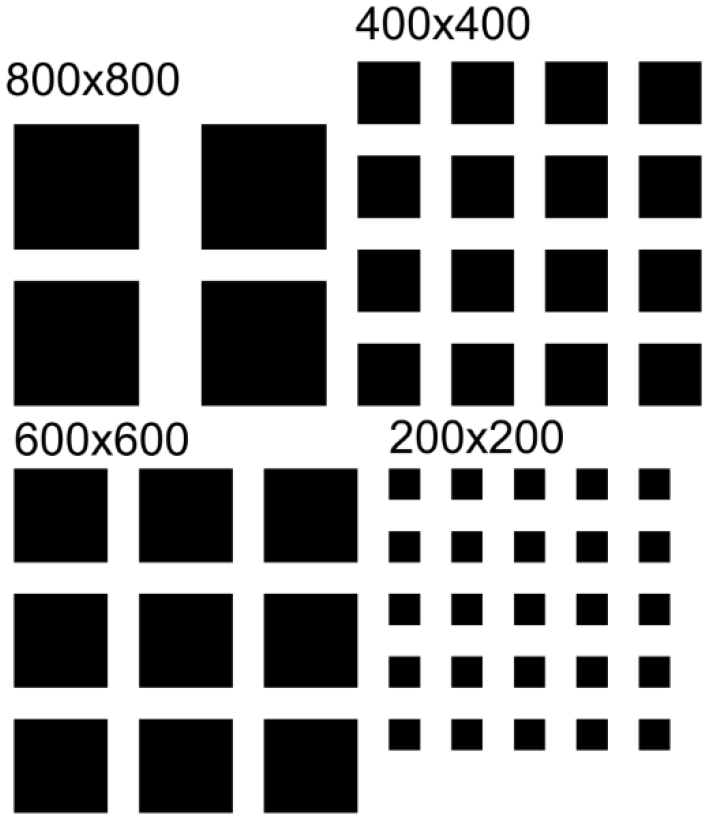
\includegraphics[width=0.4\textwidth]{Chapter3/Figs/a.png}
    \caption[Device Structure]{Device layout and dimensions of the top electrical contact.}
    \label{fig:3a}
\end{figure}

\noindent To increase adhesion, a second titanium buffer layer is placed between the top metal contact and the oxide. This adhesive layer is less than ideal since it can cause additional imperfections to migrate within the oxide. Despite this worry, research using electron energy loss spectroscopy (EELS) and transmission electron microscopy (TEM) have shown no evidence of titanium interface migration in the devices \cite{mehonic2017intrinsic}. \\

\noindent The utilisation of gold as a primary electrical contact may result in the migration of gold atoms into the oxide layer and their subsequent diffusion through the film. For instance, a study conducted into the diffusion of gold through amorphous SiOx observed the migration of gold into the oxide when the gold was held at a temperature of $390^{\circ} C$ for a period of four hours \cite{madams1974migration}. \\

\noindent Furthermore, it was established that when the gold was exposed to a temperature of $500^{\circ} C$ for a duration of two hours, it was observed to be distributed uniformly throughout the oxide layer, which had a thickness of approximately 500 nm. Nonetheless, no migration was observed at temperatures below $370^{\circ} C$. Although the diffusion of gold through silicon oxide films at elevated temperatures has been observed, this phenomenon is frequently disregarded or presumed to be non-occurring in devices utilised as resistance switching memories. \\

\noindent In the domain of electrochemical metallisation, where metallic filaments are formed between two electrodes, gold is recognised as an inert electrode \cite{kozicki2016electrochemical}. This principle is also widely accepted in the context of valence change memories [55]. In one particular instance of a device composed of gold and silver electrodes that were sandwiched between an As2S3 film, only the migration of silver was observed. \\

\noindent This migration resulted in the formation of a conductive bridge between the contacts [20]. The stability of the gold contacts within this application is assumed to be due to the fact that device operation is restricted to room temperature experiments. Alternatively, the presence and migration of a comparatively more active/mobile electrode, such as silver, may have a more significant effect on device properties.\\

\noindent It has been claimed that asymmetry in the device's construction, as well as an active and inert electrode, are necessary to identify stable switching. The molybdenum contact can be crucial as an oxygen reservoir, rapidly exchanging oxygen between the electrode and silicon oxide layer, which is similar to an active electrode, according to a recent experiment \cite{cox2021nanoscale}. The materials used for the top and bottom electrodes are different and weren't explicitly chosen for this project; rather, other group members had already picked them to create high-performance resistance switching memory. \\

\noindent The device layers remain mostly unchanged throughout the investigation. The top electrical contact is made of a different material in the experiment than the bottom electrical contact, which is made of a thin film of molybdenum. The oxide layer is made of an amorphous silicon oxide thin film. The selection of gold as the top electrical contact may cause gold atoms to diffuse through the film and migrate into the oxide. \\

\noindent Although gold has been seen to diffuse through silicon oxide layers at high temperatures, resistance switching memory frequently overlook this phenomenon or presume it does not happen. A profilometer is used to assess the thickness of the layers. To guarantee excellent conductivity throughout the device, the bottom electrode is 300 nm thick. The oxide slim film is 35nm in depth. The thickness of the top electrical contact varies depending on the substance; gold has a thickness of 110 nm, while ITO has a thickness of 50 nm.\\

\subsection[Fabrication Procedure]{Fabrication Procedure}

\noindent RF sputtering, a physical vapour deposition process, was used to deposit all of the device layers. Deposition is carried out at low pressure in a typical inert gas environment by blasting the intended material with a plasma, which causes the expulsion of atoms from the target. Depending on the gas pressure inside the chamber, the expelled atoms either follow a direct ballistic path or take a random walk until they land on the sample. A greater gas pressure will result in more collisions and an increased random walk, whereas a lower gas pressure produces a more direct ballistic trajectory. \\

\noindent  The substance being deposited, known as the target material, is initially solid. By applying a strong electric field to the sputtering gas (argon), the plasma is created. Either a DC or an AC field is possible. However, an AC field that oscillates at an RF frequency of 13.56MHz is necessary for dielectric targets like SiO2. Sputtering often results in amorphous films with sub-stoichiometric oxides. The devices' SiOx oxide has a stoichiometry of 1.9, while the film's roughness appears to be determined by the RMS roughness of the underlying molybdenum layer, which ranges from 0.9 to 1.5 nm \cite{kenyon2019interplay}. \\

\noindent After being sputtered, film thickness is measured via a contact profilometer with a 0.5nm precision. During this procedure, a diamond tip is used to make contact with the sample and scan across the surface. Utilising a feedback loop, the tip's height is adjusted to maintain a consistent force against the sample's surface as it scans, giving the measurement of the sample height. The sample's surface height changes in direct proportion to the change in tip height. Layer thicknesses of a device stack are measured in relation to one another using a staircase-like pattern that is created during production.    

\subsection[Electrical Characterisation]{Electrical Characterisation}

The amount of current passing through the device is a significant observable. This includes details on the oxide layer's bulk conductivity as well as the interface barrier heights. The difficulty, however, is in minimising any deviations or nonlinearities brought on by the measuring apparatus itself, with probe contact resistance serving as one such example. It is necessary to choose how to make contact with the device electrodes before conducting current measurements. There are essentially two methods: either the circuit is wire bonded inside a chip carrier, or the contacts are directly probed with tiny metallic probes using micromanipulators. \\

\noindent In contrast to the probe method, which can be vulnerable to sample damage brought on by the experimentalist, the wire-bonded approach has the advantage which the position of the electrical connection does not change between experiments, thermal expansion while temperature measurements will not significantly affect the contact, and there is less risk of deteriorating the device throughout characterisation. However, there is a chance that the component will be broken during the bonding procedure with wires. An ultrasonic pulse is utilised to melt a gold or aluminium wire to the device contact while applying pressure to help fuse the two metals together. It has been regularly observed that this pressure can cause internal layers to compress, leading to electric shorts between the two metal contacts and ultimately damaging the device. \\ 

\noindent The direct probing method utilising tungsten probes has been adopted instead due to the devices' design and susceptibility to break from the wire bonding procedure. The tip of the probe must be brought down carefully to prevent damage. When placing the probe into contact, a low voltage is often supplied as a test signal. To determine if the probe has made contact, the current is watched for a spike in the device current. Initially, because there is no measurable electrical current while the probe is not in touch with the device, the current oscillates around positive and negative currents at 0 amps. Once the probe makes contact with the device, the voltage that has been applied across it now causes a detectable current that matches the polarity of the applied voltage. \\


\noindent After deciding on a contact technique, the next choice is how currents will be monitored. Both a 2-wire measurement and a 4-wire measurement are frequently available as options. The sample's conductivity serves as the basis for the decision. The easiest way to measure electrical resistance is to apply a set voltage and track the total current passing through the object. Only two electrical connections are formed, thus the term "2-wire measurement" for this procedure. Ohm's Law is used to determine the device resistance by connecting a voltage source, an ammeter, and the device in series. \\

\noindent Due to the assumption that the electrical resistance is only determined by the test device, which is not true in reality where there are several sources of electrical resistance connected in series with the device, this measurement is often not correct. These include the wires connecting the test object and the voltage source, the internal resistance of the voltage source or the ammeter, and, especially, the contact resistance that develops at the point where the electrical probes and the test object meet. \\

\noindent One of the most crucial parameters to take into account when describing thin films is contact resistance, which may be reduced by placing metal contacts on the sample during manufacturing. Fortunately, the device resistance usually outweighs the electrical resistance, making this method valid in the majority of instances. However, when resistance is small, the parasitic resistances of the measuring circuit become notable and must be eliminated by using a 4-wire resistance measurement. \\

\noindent Ohm's law is still used in this configuration to calculate resistance. Instead of sourcing a voltage and monitoring a current, the device is subjected to a steady current that induces a voltage across it. Through two extra probes connected in parallel to the device, a voltmeter measures the potential decrease. It is crucial to recognise that the same contact resistance and wire resistances that plagued the 2-wire method continue to exist for all four connections. However, in this case, the high impedance of the voltmeter causes a substantially lesser current to pass through the measuring contacts. \\

\noindent The voltage recorded by the voltmeter is thought to more precisely represent the voltage drop across the device since the voltage dip across the parasitic resistance is insignificant. This occurs because the voltage produced across the contact resistance is lowered as a result of the reduced current flowing through the probes, which detect the voltage across the device. By lowering these voltages, which are induced across each probe's contact resistances and contribute mistakes into the voltage measurements, it is possible to measure the voltage across the device with more accuracy. \\

\noindent Thus, the device resistance determines whether to use a 2-wire or 4-wire resistance measurement. The devices examined in this thesis have high resistance, ranging from kiloohms to megaohms. The parasitic resistances of the measuring circuit, like the contact resistances, are insignificant at this level. The issue of measuring device currents must now be solved once the device has been attached. Again, there are a variety of techniques that might be applied; the one selected will often depend on the size of the current being measured. \\

\noindent The average current range for the devices is 100nA to 1mA, therefore a picoammeter is required to detect considerably lower currents on the order of picoamps to nanoamps. Picoammeters minimise current readings by a number of methods that differ across manufacturers. The majority of them employ a transimpedance amplifier to magnify the signal while an op-amp converts the input current to a voltage. Once again, how this is implemented differs from manufacture to manufacture and is frequently protected intellectual property that is not revealed. The equipment used in this instance is the Keithley 6430 sourcemeter, which combines a picoammeter and a low noise voltage source into a single device. \\

\noindent In some cases, the device requires the application of voltage transients that are more complex than step potentials, such as pulses or custom spike trains. In these cases, the Keithley's sampling frequency is insufficient to generate such signals. An arbitrary signal generator is used in its place to create voltage transients, and a current preamplifier is connected in series with the device to amplify device currents. In particular, the oscilloscope (Rigol DS4024) and current preamplifier (SR570) are used.

\section[Simulations]{Simulations}
